%%%%%%%%%%%%%%%%%%%%%%%%%%%%%%%%%%%%%%%%%%%%%%%%%%%%%%%%%%%%%%%%%%%%%%%%%%%%%%%
% Databricks LaTeX Beamer Presentation - Day 9
% Topic: SQL Analytics & Dashboards in Databricks
% Theme: Databricks Corporate Style
%%%%%%%%%%%%%%%%%%%%%%%%%%%%%%%%%%%%%%%%%%%%%%%%%%%%%%%%%%%%%%%%%%%%%%%%%%%%%%%

\documentclass[aspectratio=169]{beamer}

% ============================================================================
% PACKAGES
% ============================================================================
\usepackage{fontspec}
\usepackage{graphicx}
\usepackage{tikz}
\usepackage{xcolor}
\usepackage{hyperref}
\usepackage{fontawesome5}
\usepackage{booktabs}
\usepackage{array}
\usepackage{colortbl}
\usepackage{listings}
\usepackage{adjustbox}
\usepackage{multicol}

\usetikzlibrary{shapes.geometric, arrows.meta, positioning, calc, backgrounds, fit}

% ============================================================================
% DATABRICKS COLOR PALETTE
% ============================================================================
\definecolor{databricksBlue}{RGB}{41, 49, 66}
\definecolor{databricksRed}{RGB}{220, 53, 69}
\definecolor{databricksYellow}{RGB}{255, 193, 7}
\definecolor{databricksGreen}{RGB}{76, 175, 80}
\definecolor{databricksGray}{RGB}{128, 128, 128}
\definecolor{databricksLightGray}{RGB}{245, 245, 245}
\definecolor{databricksWhite}{RGB}{255, 255, 255}
\definecolor{databricksOrange}{RGB}{255, 140, 0}
\definecolor{databricksPurple}{RGB}{156, 39, 176}

% ============================================================================
% BEAMER THEME CONFIGURATION
% ============================================================================
\usetheme{default}
\usecolortheme{default}

% Remove navigation symbols
\setbeamertemplate{navigation symbols}{}

% Set colors
\setbeamercolor{structure}{fg=databricksBlue}
\setbeamercolor{title}{fg=databricksWhite}
\setbeamercolor{subtitle}{fg=databricksLightGray}
\setbeamercolor{author}{fg=databricksWhite}
\setbeamercolor{date}{fg=databricksLightGray}
\setbeamercolor{frametitle}{fg=databricksWhite,bg=databricksBlue}
\setbeamercolor{background canvas}{bg=databricksWhite}
\setbeamercolor{normal text}{fg=databricksBlue}
\setbeamercolor{itemize item}{fg=databricksBlue}
\setbeamercolor{itemize subitem}{fg=databricksRed}
\setbeamercolor{itemize subsubitem}{fg=databricksGreen}

% Set fonts
\setbeamerfont{title}{size=\Huge,series=\bfseries}
\setbeamerfont{subtitle}{size=\large}
\setbeamerfont{frametitle}{size=\Large,series=\bfseries}
\setbeamerfont{framesubtitle}{size=\normalsize}

% Itemize bullets
\setbeamertemplate{itemize item}{\textcolor{databricksBlue}{$\bullet$}}
\setbeamertemplate{itemize subitem}{\textcolor{databricksRed}{$\triangleright$}}
\setbeamertemplate{itemize subsubitem}{\textcolor{databricksGreen}{$\circ$}}

% ============================================================================
% CUSTOM FRAME TITLE
% ============================================================================
\setbeamertemplate{frametitle}{
    \begin{beamercolorbox}[wd=\paperwidth,ht=1.2cm,dp=0.3cm]{frametitle}
        \hspace{0.5cm}\insertframetitle
    \end{beamercolorbox}
}

% ============================================================================
% FOOTER CONFIGURATION
% ============================================================================
\setbeamertemplate{footline}{
    \begin{beamercolorbox}[wd=\paperwidth,ht=0.6cm,dp=0.2cm]{footline}
        
\begin{tikzpicture}[overlay, remember picture]
            \fill[databricksBlue] (0,0) rectangle (\paperwidth,0.1cm);
            % Left: Easy AI Labs
            \node[anchor=west, text=white, font=\footnotesize] at (0.5cm,0.4cm) {
                \href{https://easy-ai-labs.lovable.app/}{\textcolor{white}{Easy AI Labs}}
            };
            % Center: Yash Kavaiya
            \node[anchor=center, text=white, font=\footnotesize] at (0.5\paperwidth,0.4cm) {
                \href{https://www.linkedin.com/in/yashkavaiya}{\textcolor{white}{Yash Kavaiya}}
            };
            % Right: Gen AI Guru + Page Number
            \node[anchor=east, text=white, font=\footnotesize] at (\paperwidth-0.5cm,0.4cm) {
                \href{https://www.linkedin.com/company/genai-guru}{\textcolor{white}{Gen AI Guru}} \quad \insertframenumber/\inserttotalframenumber
            };
        \end{tikzpicture}
    \end{beamercolorbox}
}

% ============================================================================
% CODE LISTING STYLE
% ============================================================================
\lstdefinestyle{sqlstyle}{
    language=SQL,
    basicstyle=\ttfamily\scriptsize,
    keywordstyle=\color{databricksBlue}\bfseries,
    stringstyle=\color{databricksGreen},
    commentstyle=\color{databricksGray}\itshape,
    backgroundcolor=\color{databricksLightGray},
    frame=single,
    frameround=tttt,
    rulecolor=\color{databricksBlue},
    breaklines=true,
    breakatwhitespace=true,
    tabsize=2,
    showstringspaces=false,
    morekeywords={WITH, OVER, PARTITION, ROWS, BETWEEN, PRECEDING, FOLLOWING, CURRENT, ROW, UNBOUNDED, CASE, WHEN, THEN, ELSE, END, AS}
}

% ============================================================================
% TITLE PAGE INFO
% ============================================================================
\title{SQL Analytics \& Dashboards}
\subtitle{Day 9: Building Business Intelligence on Databricks}
\author{Databricks 14-Days AI Challenge}
\date{\today}

% ============================================================================
% DOCUMENT BEGIN
% ============================================================================
\begin{document}

% ============================================================================
% TITLE SLIDE
% ============================================================================
{
\setbeamertemplate{footline}{}
\begin{frame}
    \begin{tikzpicture}[overlay, remember picture]
        \fill[databricksBlue] (current page.north west) rectangle (current page.south east);
    \end{tikzpicture}
    \vspace{1cm}
    \begin{center}
        {\Huge\bfseries\textcolor{databricksWhite}{SQL Analytics \& Dashboards}\par}
        \vspace{0.5cm}
        {\Large\textcolor{databricksYellow}{Day 9: Building Business Intelligence on Databricks}\par}
        \vspace{1.5cm}
        {\large\textcolor{databricksLightGray}{Databricks 14-Days AI Challenge}\par}
        {\normalsize\textcolor{databricksGray}{\today}\par}
    \end{center}
\end{frame}
}

% ============================================================================
% TABLE OF CONTENTS
% ============================================================================
\begin{frame}{Agenda}
    \begin{columns}[T]
        \begin{column}{0.48\textwidth}
            \begin{itemize}
                \item \textcolor{databricksBlue}{\textbf{SQL Warehouses}}
                    \begin{itemize}
                        \item Types \& Architecture
                        \item Sizing Guide
                    \end{itemize}
                \item \textcolor{databricksBlue}{\textbf{Complex Analytical Queries}}
                    \begin{itemize}
                        \item Window Functions
                        \item Common Table Expressions
                    \end{itemize}
                \item \textcolor{databricksBlue}{\textbf{Dashboard Creation}}
                    \begin{itemize}
                        \item Visualization Types
                        \item Design Principles
                    \end{itemize}
            \end{itemize}
        \end{column}
        \begin{column}{0.48\textwidth}
            \begin{itemize}
                \item \textcolor{databricksBlue}{\textbf{Visualizations \& Filters}}
                    \begin{itemize}
                        \item Filter Implementation
                        \item Scheduled Refresh
                    \end{itemize}
                \item \textcolor{databricksBlue}{\textbf{Practical Tasks}}
                    \begin{itemize}
                        \item 7-Day Moving Average
                        \item Conversion Funnel
                        \item Customer Tier Segmentation
                    \end{itemize}
                \item \textcolor{databricksBlue}{\textbf{Best Practices}}
            \end{itemize}
        \end{column}
    \end{columns}
\end{frame}

% ============================================================================
% INTRODUCTION
% ============================================================================
\begin{frame}{Introduction to SQL Analytics}
    \begin{columns}[T]
        \begin{column}{0.55\textwidth}
            \textcolor{databricksBlue}{\textbf{What is SQL Analytics?}}
            \vspace{0.3cm}
            
            A powerful environment for:
            \begin{itemize}
                \item Running \textbf{analytical queries}
                \item Building \textbf{interactive dashboards}
                \item Gaining \textbf{insights} from your data lakehouse
            \end{itemize}
            
            \vspace{0.5cm}
            \textcolor{databricksRed}{\textbf{Why It Matters:}}
            \begin{itemize}
                \item Enables analysts without Spark knowledge
                \item Familiar SQL interface
                \item Direct lakehouse integration
                \item Real-time dashboard capabilities
            \end{itemize}
        \end{column}
        \begin{column}{0.42\textwidth}
            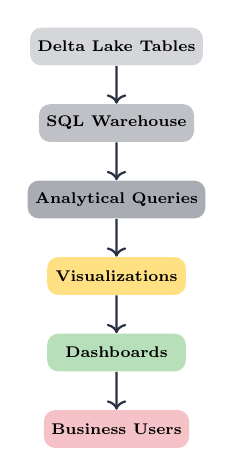
\begin{tikzpicture}[node distance=0.6cm, scale=0.8, transform shape]
                \tikzstyle{box} = [rectangle, rounded corners, minimum width=2.2cm, minimum height=0.6cm, text centered, font=\scriptsize\bfseries]
                \tikzstyle{arrow} = [->, thick, databricksBlue]
                
                \node[box, fill=databricksBlue!20] (delta) {Delta Lake Tables};
                \node[box, fill=databricksBlue!30, below=of delta] (warehouse) {SQL Warehouse};
                \node[box, fill=databricksBlue!40, below=of warehouse] (queries) {Analytical Queries};
                \node[box, fill=databricksYellow!50, below=of queries] (viz) {Visualizations};
                \node[box, fill=databricksGreen!40, below=of viz] (dash) {Dashboards};
                \node[box, fill=databricksRed!30, below=of dash] (users) {Business Users};
                
                \draw[arrow] (delta) -- (warehouse);
                \draw[arrow] (warehouse) -- (queries);
                \draw[arrow] (queries) -- (viz);
                \draw[arrow] (viz) -- (dash);
                \draw[arrow] (dash) -- (users);
            \end{tikzpicture}
        \end{column}
    \end{columns}
\end{frame}

% ============================================================================
% SQL WAREHOUSES
% ============================================================================
\begin{frame}{SQL Warehouses Overview}
    \textcolor{databricksBlue}{\textbf{What is a SQL Warehouse?}}
    The \textbf{compute resource} that executes SQL queries against Delta Lake tables.
    \begin{center}
    \begin{tabular}{>{\columncolor{databricksBlue!10}}l l l l}
        \toprule
        \rowcolor{databricksBlue}
        \textcolor{white}{\textbf{Type}} & \textcolor{white}{\textbf{Description}} & \textcolor{white}{\textbf{Best Use Case}} & \textcolor{white}{\textbf{Cost Model}} \\
        \midrule
        \textbf{Serverless} & Fully managed, instant startup & Ad-hoc queries & Pay per query \\
        \textbf{Pro} & Provisioned with advanced features & Production dashboards & Pay per hour \\
        \textbf{Classic} & Basic provisioned clusters & Development, testing & Pay per hour \\
        \bottomrule
    \end{tabular}
    \end{center}
    \textcolor{databricksGreen}{\textbf{Key Benefits:}}
    \begin{itemize}
        \item \textbf{Separation of compute and storage} -- Scale independently
        \item \textbf{Photon Engine} -- Vectorized query acceleration
        \item \textbf{Auto-scaling \& Auto-stop} -- Cost optimization
    \end{itemize}
\end{frame}

% ============================================================================
% SQL WAREHOUSE ARCHITECTURE
% ============================================================================
\begin{frame}{SQL Warehouse Architecture}
    \begin{center}
    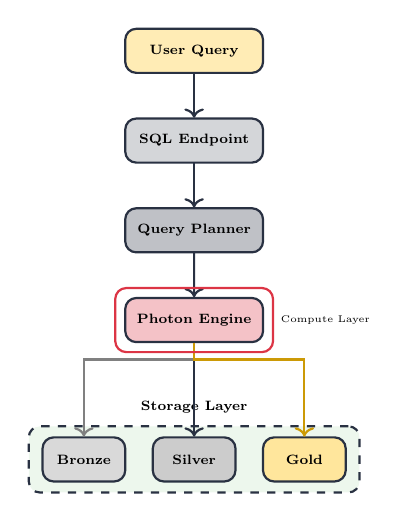
\begin{tikzpicture}[node distance=0.8cm, scale=0.7, transform shape]
        \tikzstyle{box} = [rectangle, rounded corners, minimum width=2.5cm, minimum height=0.8cm, text centered, font=\scriptsize\bfseries, draw=databricksBlue, thick]
        \tikzstyle{layer} = [rectangle, rounded corners, minimum width=6cm, minimum height=1.2cm, draw=databricksBlue, dashed, thick]
        \tikzstyle{arrow} = [->, thick, databricksBlue]
        
        \node[box, fill=databricksYellow!30] (query) {User Query};
        \node[box, fill=databricksBlue!20, below=of query] (endpoint) {SQL Endpoint};
        \node[box, fill=databricksBlue!30, below=of endpoint] (planner) {Query Planner};
        \node[box, fill=databricksRed!30, below=of planner] (photon) {Photon Engine};
        
        \node[layer, below=1.5cm of photon, fill=databricksGreen!10] (storage) {};
        \node[above=0.1cm] at (storage.north) {\scriptsize\textbf{Storage Layer}};
        
        \node[box, fill=databricksGray!30, minimum width=1.5cm] at ([xshift=-2cm]storage.center) (bronze) {Bronze};
        \node[box, fill=databricksGray!40, minimum width=1.5cm] at (storage.center) (silver) {Silver};
        \node[box, fill=databricksYellow!40, minimum width=1.5cm] at ([xshift=2cm]storage.center) (gold) {Gold};
        
        \draw[arrow] (query) -- (endpoint);
        \draw[arrow] (endpoint) -- (planner);
        \draw[arrow] (planner) -- (photon);
        \draw[arrow] (photon) -- (silver);
        \draw[arrow, databricksGray] (photon.south) -- ++(0,-0.3) -| (bronze.north);
        \draw[arrow, databricksYellow!80!black] (photon.south) -- ++(0,-0.3) -| (gold.north);
        
        \node[rectangle, rounded corners, draw=databricksRed, thick, fit=(photon), label={[font=\tiny]right:Compute Layer}] {};
    \end{tikzpicture}
    \end{center}
\end{frame}

% ============================================================================
% WAREHOUSE SIZING
% ============================================================================
\begin{frame}{Warehouse Sizing Guide}
    \begin{columns}[T]
        \begin{column}{0.55\textwidth}
            \textcolor{databricksBlue}{\textbf{Configuration Parameters:}}
           
            
            \begin{tabular}{>{\columncolor{databricksBlue!10}}l l}
                \toprule
                \rowcolor{databricksBlue}
                \textcolor{white}{\textbf{Parameter}} & \textcolor{white}{\textbf{Recommendation}} \\
                \midrule
                \textbf{Name} & Descriptive (e.g., \texttt{analytics\_prod}) \\
                \textbf{Cluster Size} & Start small, scale up \\
                \textbf{Min/Max Clusters} & Min=1, Max=based on users \\
                \textbf{Auto Stop} & 10-30 min for dev \\
                \bottomrule
            \end{tabular}
        \end{column}
        \begin{column}{0.42\textwidth}
            \textcolor{databricksRed}{\textbf{Size Reference:}}
          
            \begin{tabular}{l c c}
                \toprule
                \rowcolor{databricksBlue}
                \textcolor{white}{\textbf{Size}} & \textcolor{white}{\textbf{DBU/Hr}} & \textcolor{white}{\textbf{Memory}} \\
                \midrule
                2X-Small & 2 & 16 GB \\
                X-Small & 4 & 32 GB \\
                Small & 8 & 64 GB \\
                Medium & 16 & 128 GB \\
                Large & 32 & 256 GB \\
                \bottomrule
            \end{tabular}
        \end{column}
    \end{columns}

    \begin{center}
        \colorbox{databricksYellow!20}{\parbox{0.8\textwidth}{\centering
            \textcolor{databricksBlue}{\faLightbulb} \textbf{Tip:} Start with 2X-Small and scale based on query performance metrics
        }}
    \end{center}
\end{frame}

% ============================================================================
% WINDOW FUNCTIONS
% ============================================================================
\begin{frame}[fragile]{Understanding Window Functions}
    \begin{columns}[T]
        \begin{column}{0.55\textwidth}
            \textcolor{databricksBlue}{\textbf{What are Window Functions?}}
            \vspace{0.2cm}
            
            Perform calculations across a \textbf{set of related rows} while retaining individual rows.
            
            \vspace{0.3cm}
            \textcolor{databricksRed}{\textbf{General Syntax:}}
            \begin{lstlisting}[style=sqlstyle, basicstyle=\ttfamily\tiny]
function_name(expression) OVER (
    [PARTITION BY partition_expr]
    [ORDER BY order_expr]
    [frame_clause]
)
            \end{lstlisting}
            
            \vspace{0.3cm}
            \textcolor{databricksGreen}{\textbf{Frame Clause Example:}}
            \begin{lstlisting}[style=sqlstyle, basicstyle=\ttfamily\tiny]
ROWS BETWEEN 6 PRECEDING AND CURRENT ROW
            \end{lstlisting}
            Include current row + 6 previous rows (7 total)
        \end{column}
        \begin{column}{0.42\textwidth}
            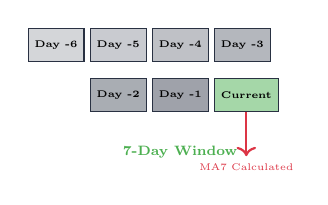
\begin{tikzpicture}[scale=0.7, transform shape]
                \tikzstyle{day} = [rectangle, minimum width=1cm, minimum height=0.6cm, text centered, font=\tiny\bfseries, draw=databricksBlue]
                
                \node[day, fill=databricksBlue!20] (d1) at (0,0) {Day -6};
                \node[day, fill=databricksBlue!25, right=0.1cm of d1] (d2) {Day -5};
                \node[day, fill=databricksBlue!30, right=0.1cm of d2] (d3) {Day -4};
                \node[day, fill=databricksBlue!35, right=0.1cm of d3] (d4) {Day -3};
                \node[day, fill=databricksBlue!40, below=0.3cm of d2] (d5) {Day -2};
                \node[day, fill=databricksBlue!45, right=0.1cm of d5] (d6) {Day -1};
                \node[day, fill=databricksGreen!50, right=0.1cm of d6] (d7) {Current};
                
                \node[below=0.5cm of d6, font=\scriptsize] {\textcolor{databricksGreen}{\textbf{7-Day Window}}};
                
                \draw[thick, databricksRed, ->] (d7.south) -- ++(0,-0.8) node[below, font=\tiny] {MA7 Calculated};
            \end{tikzpicture}
        \end{column}
    \end{columns}
\end{frame}

% ============================================================================
% COMMON WINDOW FUNCTIONS
% ============================================================================
\begin{frame}{Common Window Functions}
    \begin{center}
    \begin{tabular}{>{\columncolor{databricksBlue!10}}l l l}
        \toprule
        \rowcolor{databricksBlue}
        \textcolor{white}{\textbf{Function}} & \textcolor{white}{\textbf{Purpose}} & \textcolor{white}{\textbf{Example Use Case}} \\
        \midrule
        \texttt{ROW\_NUMBER()} & Assigns unique sequential integers & Ranking products \\
        \texttt{RANK()} & Assigns rank with gaps for ties & Leaderboards \\
        \texttt{DENSE\_RANK()} & Assigns rank without gaps & Competition rankings \\
        \texttt{LAG()} & Accesses previous row value & Day-over-day comparison \\
        \texttt{LEAD()} & Accesses next row value & Forecasting trends \\
        \texttt{SUM() OVER} & Running total & Cumulative revenue \\
        \texttt{AVG() OVER} & Moving average & Smoothing trends \\
        \texttt{FIRST\_VALUE()} & First value in window & Baseline comparisons \\
        \texttt{LAST\_VALUE()} & Last value in window & Latest status \\
        \bottomrule
    \end{tabular}
    \end{center}
\end{frame}

% ============================================================================
% CTEs
% ============================================================================
\begin{frame}[fragile]{Common Table Expressions (CTEs)}
    \begin{columns}[T]
        \begin{column}{0.55\textwidth}
            \textcolor{databricksBlue}{\textbf{What are CTEs?}}      
            Temporary named result sets that exist only for the duration of the query.
            
            \vspace{0.3cm}
            \begin{lstlisting}[style=sqlstyle, basicstyle=\ttfamily\tiny]
WITH cte_name AS (
    -- First query
    SELECT ...
),
another_cte AS (
    -- Can reference previous CTEs
    SELECT ... FROM cte_name
)
SELECT * FROM another_cte;
            \end{lstlisting}
        \end{column}
        \begin{column}{0.42\textwidth}
            \textcolor{databricksGreen}{\textbf{Benefits:}}
            \vspace{0.2cm}
            
            \begin{itemize}
                \item \textcolor{databricksBlue}{$\bullet$} Improve query \textbf{readability}
                \item \textcolor{databricksBlue}{$\bullet$} Allow \textbf{recursive} queries
                \item \textcolor{databricksBlue}{$\bullet$} Can be referenced \textbf{multiple times}
                \item \textcolor{databricksBlue}{$\bullet$} Easier to \textbf{debug} complex logic
            \end{itemize}
            \colorbox{databricksYellow!20}{\parbox{0.9\columnwidth}{\centering
                \scriptsize\textcolor{databricksBlue}{\faLightbulb} Break complex queries into logical steps
            }}
        \end{column}
    \end{columns}
\end{frame}

% ============================================================================
% DASHBOARD COMPONENTS
% ============================================================================
\begin{frame}{Dashboard Components}
    \begin{center}
    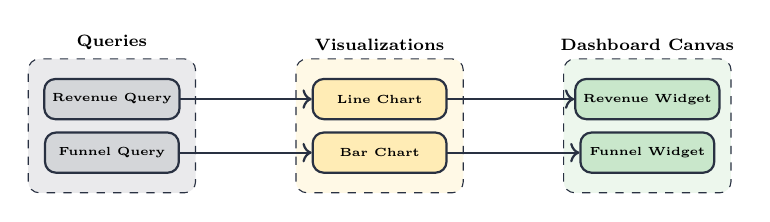
\begin{tikzpicture}[node distance=0.6cm, scale=0.85, transform shape]
        \tikzstyle{box} = [rectangle, rounded corners, minimum width=2cm, minimum height=0.6cm, text centered, font=\tiny\bfseries, draw=databricksBlue, thick]
        \tikzstyle{group} = [rectangle, rounded corners, minimum width=2.5cm, minimum height=2cm, draw=databricksBlue, dashed]
        \tikzstyle{arrow} = [->, thick, databricksBlue]
        
        % Queries
        \node[group, fill=databricksBlue!10, label={[font=\scriptsize\bfseries]above:Queries}] (qgroup) at (0,0) {};
        \node[box, fill=databricksBlue!20] (q1) at (0,0.4) {Revenue Query};
        \node[box, fill=databricksBlue!20] (q2) at (0,-0.4) {Funnel Query};
        
        % Visualizations
        \node[group, fill=databricksYellow!10, label={[font=\scriptsize\bfseries]above:Visualizations}] (vgroup) at (4,0) {};
        \node[box, fill=databricksYellow!30] (v1) at (4,0.4) {Line Chart};
        \node[box, fill=databricksYellow!30] (v2) at (4,-0.4) {Bar Chart};
        
        % Dashboard
        \node[group, fill=databricksGreen!10, label={[font=\scriptsize\bfseries]above:Dashboard Canvas}] (dgroup) at (8,0) {};
        \node[box, fill=databricksGreen!30] (d1) at (8,0.4) {Revenue Widget};
        \node[box, fill=databricksGreen!30] (d2) at (8,-0.4) {Funnel Widget};
        
        \draw[arrow] (q1) -- (v1);
        \draw[arrow] (q2) -- (v2);
        \draw[arrow] (v1) -- (d1);
        \draw[arrow] (v2) -- (d2);
    \end{tikzpicture}
    \end{center}

    \textcolor{databricksBlue}{\textbf{Dashboard = Multiple visualizations (widgets) arranged on a canvas}}
    \textcolor{databricksRed}{\textbf{Each visualization is powered by a SQL query}}
\end{frame}

% ============================================================================
% VISUALIZATION TYPES
% ============================================================================
\begin{frame}{Visualization Types}
    \begin{center}
    \begin{tabular}{>{\columncolor{databricksBlue!10}}l l l}
        \toprule
        \rowcolor{databricksBlue}
        \textcolor{white}{\textbf{Visualization}} & \textcolor{white}{\textbf{Best For}} & \textcolor{white}{\textbf{Example}} \\
        \midrule
        \textbf{Line Chart} & Trends over time & Revenue over months \\
        \textbf{Bar Chart} & Comparing categories & Sales by region \\
        \textbf{Pie/Donut Chart} & Part-to-whole relationships & Market share \\
        \textbf{Counter} & Single KPI display & Total revenue \\
        \textbf{Table} & Detailed data display & Top products list \\
        \textbf{Funnel} & Stage-based conversion & Purchase funnel \\
        \textbf{Scatter Plot} & Correlation analysis & Price vs. quantity \\
        \textbf{Heatmap} & Matrix relationships & Activity by day/hour \\
        \bottomrule
    \end{tabular}
    \end{center}
    \textcolor{databricksGreen}{\textbf{Design Principles:}}
    \begin{multicols}{2}
        \begin{itemize}
            \item \textbf{Hierarchy:} Important metrics at top-left
            \item \textbf{Grouping:} Related vizs together
            \item \textbf{Context:} Provide comparison points
            \item \textbf{Clarity:} One question per widget
        \end{itemize}
    \end{multicols}
\end{frame}

% ============================================================================
% FILTERS
% ============================================================================
\begin{frame}[fragile]{Filters \& Interactivity}
    \begin{columns}[T]
        \begin{column}{0.48\textwidth}
            \textcolor{databricksBlue}{\textbf{Filter Types:}}         
            \begin{tabular}{l l}
                \toprule
                \rowcolor{databricksBlue}
                \textcolor{white}{\textbf{Type}} & \textcolor{white}{\textbf{Example}} \\
                \midrule
                Dropdown & Category selection \\
                Date Range & Report period \\
                Text & Search by name \\
                Query-based & Dynamic list \\
                \bottomrule
            \end{tabular}
            \textcolor{databricksRed}{\textbf{Implementation:}}
            \begin{lstlisting}[style=sqlstyle, basicstyle=\ttfamily\tiny]
SELECT * FROM gold.products
WHERE category_code = 
      '{{ category_filter }}'
AND event_date BETWEEN 
    '{{ start_date }}' 
    AND '{{ end_date }}'
            \end{lstlisting}
        \end{column}
        \begin{column}{0.48\textwidth}
            \textcolor{databricksGreen}{\textbf{Scheduled Refresh:}}
            \begin{tabular}{l l}
                \toprule
                \rowcolor{databricksBlue}
                \textcolor{white}{\textbf{Interval}} & \textcolor{white}{\textbf{Use Case}} \\
                \midrule
                1 minute & Real-time monitoring \\
                1 hour & Operational dashboards \\
                Daily & Executive reports \\
                Weekly & Summary dashboards \\
                \bottomrule
            \end{tabular}
            \colorbox{databricksYellow!20}{\parbox{0.9\columnwidth}{\centering
                \scriptsize\textcolor{databricksBlue}{\faExclamationTriangle} More frequent = Higher cost
            }}
        \end{column}
    \end{columns}
\end{frame}

% ============================================================================
% TASK 1: MOVING AVERAGE
% ============================================================================
\begin{frame}[fragile]{Task 1: Revenue with 7-Day Moving Average}
    \textcolor{databricksBlue}{\textbf{Goal:}} Calculate daily revenue and smooth with 7-day moving average

    \begin{columns}[T]
        \begin{column}{0.55\textwidth}
            \begin{lstlisting}[style=sqlstyle, basicstyle=\ttfamily\tiny]
-- Revenue with 7-day moving average
WITH daily AS (
    SELECT 
        event_date,
        SUM(revenue) as rev
    FROM gold.products
    GROUP BY event_date
)
SELECT 
    event_date,
    rev,
    AVG(rev) OVER (
        ORDER BY event_date 
        ROWS BETWEEN 6 PRECEDING 
             AND CURRENT ROW
    ) as ma7
FROM daily;
            \end{lstlisting}
        \end{column}
        \begin{column}{0.42\textwidth}
            \textcolor{databricksGreen}{\textbf{Mathematical Formula:}}
            \vspace{0.2cm}
            
            $$MA_7(t) = \frac{1}{7} \sum_{i=0}^{6} R_{t-i}$$
            
            \vspace{0.2cm}
            Where:
            \begin{itemize}
                \item $MA_7(t)$ = 7-day MA at time $t$
                \item $R_{t-i}$ = Revenue on day $t-i$
            \end{itemize}
            \textcolor{databricksRed}{\textbf{Why 7-Day?}}
            \begin{itemize}
                \item \textcolor{databricksRed}{$\triangleright$} Smooths daily volatility
                \item \textcolor{databricksRed}{$\triangleright$} Captures weekly patterns
                \item \textcolor{databricksRed}{$\triangleright$} Identifies trends
            \end{itemize}
        \end{column}
    \end{columns}
\end{frame}

% ============================================================================
% TASK 2: CONVERSION FUNNEL
% ============================================================================
\begin{frame}[fragile]{Task 2: Conversion Funnel Analysis}
    \textcolor{databricksBlue}{\textbf{Goal:}} Measure how effectively categories convert views into purchases
    
    \begin{columns}[T]
        \begin{column}{0.52\textwidth}
            \begin{lstlisting}[style=sqlstyle, basicstyle=\ttfamily\tiny]
-- Conversion funnel
SELECT 
    category_code,
    SUM(views) as views,
    SUM(purchases) as purchases,
    ROUND(SUM(purchases) * 100.0 
          / SUM(views), 2) 
        as conversion_rate
FROM gold.products
GROUP BY category_code;
            \end{lstlisting}
            \textcolor{databricksGreen}{\textbf{Formula:}}
            $$\text{Rate} = \frac{\text{Purchases}}{\text{Views}} \times 100$$
        \end{column}
        \begin{column}{0.45\textwidth}
            \textcolor{databricksRed}{\textbf{Interpreting Results:}}
            
            \begin{tabular}{l l}
                \toprule
                \rowcolor{databricksBlue}
                \textcolor{white}{\textbf{Rate}} & \textcolor{white}{\textbf{Status}} \\
                \midrule
                < 1\% & Poor \\
                1-3\% & Average \\
                3-5\% & Good \\
                > 5\% & Excellent \\
                \bottomrule
            \end{tabular}
            \colorbox{databricksYellow!20}{\parbox{0.9\columnwidth}{\centering
                \scriptsize Use \texttt{100.0} for float division!
            }}
        \end{column}
    \end{columns}
\end{frame}

% ============================================================================
% TASK 3: CUSTOMER TIERS
% ============================================================================
\begin{frame}[fragile]{Task 3: Customer Tier Segmentation}
    \textcolor{databricksBlue}{\textbf{Goal:}} Segment customers into tiers based on purchase frequency
    \begin{lstlisting}[style=sqlstyle, basicstyle=\ttfamily\tiny]
SELECT 
    CASE 
        WHEN cnt >= 10 THEN 'VIP'
        WHEN cnt >= 5 THEN 'Loyal'
        ELSE 'Regular'
    END as tier,
    COUNT(*) as customers,
    AVG(total_spent) as avg_ltv
FROM (
    SELECT user_id, COUNT(*) cnt, SUM(price) total_spent
    FROM silver.events WHERE event_type = 'purchase' GROUP BY user_id
) 
GROUP BY tier;
    \end{lstlisting}
    \begin{columns}[T]
        \begin{column}{0.48\textwidth}
            \textcolor{databricksGreen}{\textbf{Tier Definitions:}}
            \begin{tabular}{l l}
                \toprule
                \textbf{VIP} & 10+ purchases \\
                \textbf{Loyal} & 5-9 purchases \\
                \textbf{Regular} & 1-4 purchases \\
                \bottomrule
            \end{tabular}
        \end{column}
        \begin{column}{0.48\textwidth}
            \textcolor{databricksRed}{\textbf{LTV Formula:}}
            $$\text{Avg LTV} = \frac{\sum \text{TotalSpent}}{n}$$
        \end{column}
    \end{columns}
\end{frame}

% ============================================================================
% BEST PRACTICES
% ============================================================================
\begin{frame}{Best Practices}
    \begin{columns}[T]
        \begin{column}{0.48\textwidth}
            \textcolor{databricksBlue}{\textbf{Query Optimization:}}
            \begin{itemize}
                \item \textbf{Use Appropriate Data Layers:}
                    \begin{itemize}
                        \item Bronze: Avoid for analytics
                        \item Silver: Detailed analysis
                        \item \textcolor{databricksYellow}{\textbf{Gold: Best for dashboards}}
                    \end{itemize}
                \item \textbf{Leverage Partitioning}
                \item \textbf{Use Delta Lake Features:}
                    \begin{itemize}
                        \item Z-ordering
                        \item OPTIMIZE
                        \item VACUUM
                    \end{itemize}
            \end{itemize}
        \end{column}
        \begin{column}{0.48\textwidth}
            \textcolor{databricksRed}{\textbf{Cost Management:}}  
            \begin{itemize}
                \item \textcolor{databricksBlue}{$\bullet$} \textbf{Right-size} warehouses
                \item \textcolor{databricksBlue}{$\bullet$} Use \textbf{auto-stop}
                \item \textcolor{databricksBlue}{$\bullet$} \textbf{Monitor} query history
                \item \textcolor{databricksBlue}{$\bullet$} Schedule during \textbf{off-peak}
            \end{itemize}
            \textcolor{databricksGreen}{\textbf{Dashboard Performance:}}
            \begin{itemize}
                \item Pre-aggregate data
                \item Limit result sets
                \item Enable query caching
            \end{itemize}
        \end{column}
    \end{columns}
\end{frame}

% ============================================================================
% QUICK REFERENCE
% ============================================================================
\begin{frame}[fragile]{Quick Reference: Useful SQL Patterns}
    \begin{columns}[T]
        \begin{column}{0.48\textwidth}
            \textcolor{databricksBlue}{\textbf{Running Total:}}
            \begin{lstlisting}[style=sqlstyle, basicstyle=\ttfamily\tiny]
SUM(amount) OVER (
    ORDER BY date 
    ROWS UNBOUNDED PRECEDING)
            \end{lstlisting}
            \textcolor{databricksRed}{\textbf{Rank within Group:}}
            \begin{lstlisting}[style=sqlstyle, basicstyle=\ttfamily\tiny]
ROW_NUMBER() OVER (
    PARTITION BY category 
    ORDER BY sales DESC)
            \end{lstlisting}
            \textcolor{databricksGreen}{\textbf{Year-over-Year:}}
            \begin{lstlisting}[style=sqlstyle, basicstyle=\ttfamily\tiny]
LAG(revenue, 12) OVER (
    ORDER BY month) 
    as prev_year_revenue
            \end{lstlisting}
        \end{column}
        \begin{column}{0.48\textwidth}
            \textcolor{databricksPurple}{\textbf{Percent of Total:}}
            \begin{lstlisting}[style=sqlstyle, basicstyle=\ttfamily\tiny]
revenue * 100.0 / 
    SUM(revenue) OVER () 
    as pct_of_total
            \end{lstlisting}
            \textcolor{databricksOrange}{\textbf{Filter Parameters:}}
            \begin{tabular}{l}
                \toprule
                \texttt{WHERE col = '\{\{ param \}\}'} \\
                \texttt{WHERE col IN (\{\{ param \}\})} \\
                \texttt{WHERE date BETWEEN ...} \\
                \bottomrule
            \end{tabular}
        \end{column}
    \end{columns}
\end{frame}

% ============================================================================
% SUMMARY
% ============================================================================
\begin{frame}{Summary}
    \begin{center}
    \begin{tabular}{>{\columncolor{databricksBlue!10}}l l}
        \toprule
        \rowcolor{databricksBlue}
        \textcolor{white}{\textbf{Component}} & \textcolor{white}{\textbf{Purpose}} \\
        \midrule
        \textbf{SQL Warehouse} & Compute engine for query execution \\
        \textbf{Query Editor} & Write and test SQL queries \\
        \textbf{Visualizations} & Transform data into charts \\
        \textbf{Dashboards} & Combine visualizations into reports \\
        \textbf{Filters} & Enable interactive exploration \\
        \textbf{Scheduling} & Automate refresh cycles \\
        \bottomrule
    \end{tabular}
    \end{center}
    \textcolor{databricksBlue}{\textbf{Key Patterns Covered:}}
    \begin{enumerate}
        \item \textcolor{databricksRed}{\textbf{Moving Average}} -- Trend analysis with window functions
        \item \textcolor{databricksGreen}{\textbf{Conversion Funnel}} -- Performance metrics with aggregation
        \item \textcolor{databricksYellow}{\textbf{Customer Tiers}} -- Segmentation with CASE statements
    \end{enumerate}
\end{frame}

% ============================================================================
% THANK YOU SLIDE
% ============================================================================
{
\setbeamertemplate{footline}{}
\begin{frame}
    \begin{tikzpicture}[overlay, remember picture]
        \fill[databricksBlue] (current page.north west) rectangle (current page.south east);
    \end{tikzpicture}
    \begin{center}
        \vspace{2cm}
        {\Huge\bfseries\textcolor{databricksWhite}{Thank You!}\par}
        \vspace{1cm}
        {\Large\textcolor{databricksYellow}{Day 9 Complete}\par}
        \vspace{0.5cm}
        {\large\textcolor{databricksLightGray}{SQL Analytics \& Dashboards in Databricks}\par}
        \vspace{1.5cm}
        {\normalsize\textcolor{databricksGray}{
            \href{https://www.linkedin.com/in/yashkavaiya}{\faLinkedin\ Yash Kavaiya} \quad | \quad
            \href{https://www.linkedin.com/company/genai-guru}{\faBuilding\ Gen AI Guru}
        }\par}
    \end{center}
\end{frame}
}

\end{document}
